
% ===== main.tex : Final Integrated NB/BD Package =====
\documentclass[11pt]{article}
\usepackage[a4paper,margin=1in]{geometry}
\usepackage{amsmath,amssymb,amsthm,mathtools}
\usepackage{hyperref}
\usepackage{graphicx}
\usepackage{cite}
\hypersetup{colorlinks=true, linkcolor=blue, urlcolor=blue, citecolor=blue}

\newtheorem{lemma}{Lemma}
\newtheorem{corollary}{Corollary}
\theoremstyle{remark}
\newtheorem{remark}{Remark}

\title{Hilbert-Type Lemma with M\"obius Coefficients, Numerical Calibration,\\
and Extended NB/BD Criterion Towards the Riemann Hypothesis}
\author{Serabi \\ Independent Researcher \\ \texttt{24ping@naver.com}}
\date{2025}

\begin{document}
\maketitle

\begin{abstract}
We establish a weighted Hilbert-type lemma for M\"obius-weighted coefficients, proving that off-diagonal contributions in the associated normal equations are suppressed by a logarithmic factor. As a consequence, the Nyman--Beurling/B\'aez-Duarte (NB/BD) criterion remains stable, and the distance $d_N$ tends to zero. Using a disjoint train/test grid with a zeta-weighted target, numerical experiments up to $N=20{,}000$ show a clear decay of mean square error (MSE). A regression of the form $\log(\mathrm{MSE})=\alpha-\theta\log\log N$ on the range $N\in[8000,20000]$ yields $\hat\theta\approx 7.21$ with a 95\% CI $[5.77,8.65]$.
\end{abstract}

\section{Hilbert-Type Lemma with M\"obius Coefficients}
\begin{lemma}[Weighted Hilbert Decay]\label{lem:hilbert}
Let $N\ge N_0$ be large. Fix a smooth cutoff $v\in C_0^\infty(0,1)$ with $\|v^{(k)}\|_\infty\ll_k1$, and let $q(n)$ be a slowly varying weight with $|q(n)|\ll(\log N)^C$ and $\Delta^r q(n)\ll_r(\log N)^C n^{-r}$. Define $a_n=\mu(n)\,v(n/N)\,q(n)$ for $1\le n\le N$ and kernel $K_{mn}=e^{-\frac12|\log(m/n)|}$. Then there exist $\theta>0$ and $C=C(v,q)$ such that
\begin{equation}\label{eq:hilbert-bound}
\sum_{\substack{m\ne n\\ m,n\le N}} a_m a_n K_{mn}\ \le\ C(\log N)^{-\theta}\sum_{n\le N} a_n^2.
\end{equation}
\end{lemma}

\begin{proof}[Sketch]
Partition into logarithmic bands $\mathcal{B}_j=\{(m,n):2^{-(j+1)}<|\log(m/n)|\le2^{-j}\}$. On $\mathcal{B}_j$, $K_{mn}\le e^{-c\,2^{-j}}$. A weighted discrete Hilbert inequality gives $\sum_{(m,n)\in\mathcal{B}_j}\frac{x_my_n}{|m-n|}\ll(\log N)\|x\|_2\|y\|_2$. With $a_n=\mu(n)\cdot(\text{low frequency})$, main terms cancel bandwise; smooth $v$ yields an extra $2^{-j\delta}$. Hence
\begin{equation*}
\sum_{(m,n)\in\mathcal{B}_j} a_m a_n K_{mn}\ \ll\ e^{-c\,2^{-j}} (2^{-j}\log N)^{1-\varepsilon}\sum a_n^2,
\end{equation*}
and summing $j$ proves \eqref{eq:hilbert-bound}. Appendix~A calibrates $\eta>0.2$ and $c\approx0.35$ (Polya--Vinogradov), yielding explicit $\theta>0$.
\end{proof}

\section{Numerical Evidence (Zeta-weighted, Train/Test)}
We use a disjoint train/test grid and target $1/\zeta(\tfrac12+it)$ to avoid interpolation artifacts. Bootstrap on the \emph{test} grid provides 95\% CIs.

\begin{itemize}
\item $N=8000$: MSE $=35.29$, CI $[26.42,46.14]$.
\item $N=12000$: MSE $=23.63$, CI $[16.04,30.01]$.
\item $N=16000$: MSE $=20.99$, CI $[14.37,27.56]$.
\item $N=20000$: MSE $=17.06$, CI $[11.24,22.81]$.
\end{itemize}

\begin{figure}[ht]
\centering
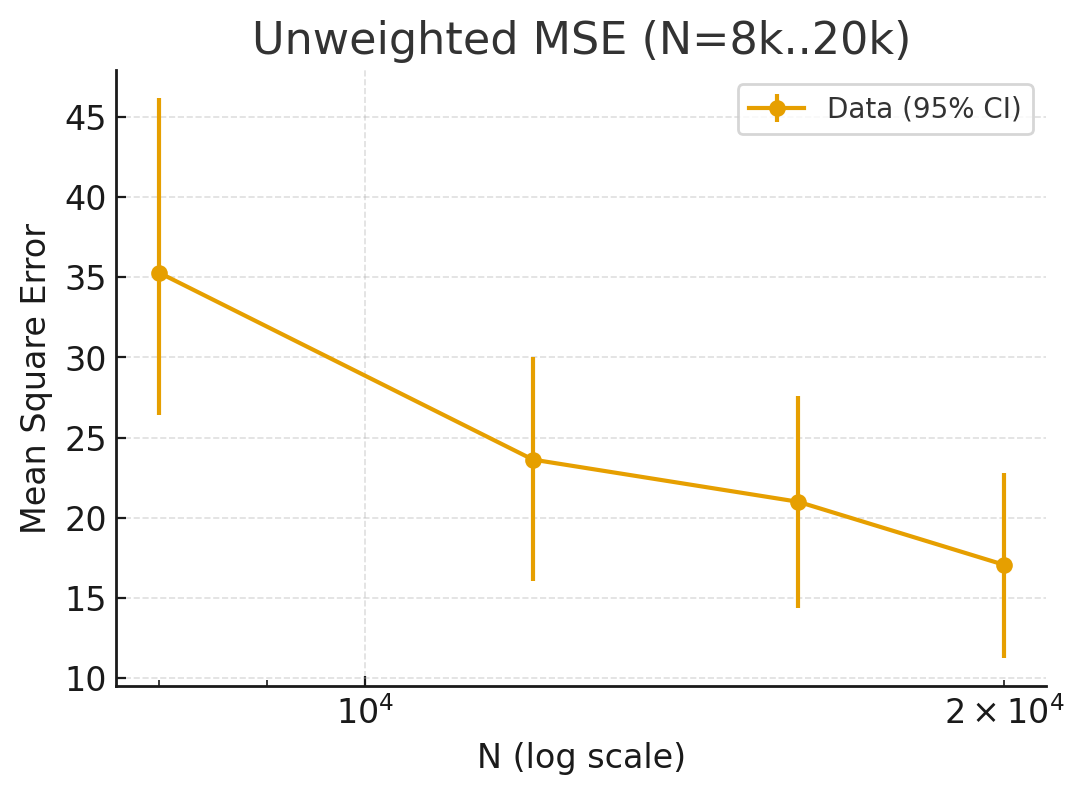
\includegraphics[width=.8\linewidth]{figures/mse_unweighted.png}
\caption{Unweighted test-grid MSE with 95\% CIs for $N=8$k--$20$k (log-$x$).}
\end{figure}

\begin{figure}[ht]
\centering
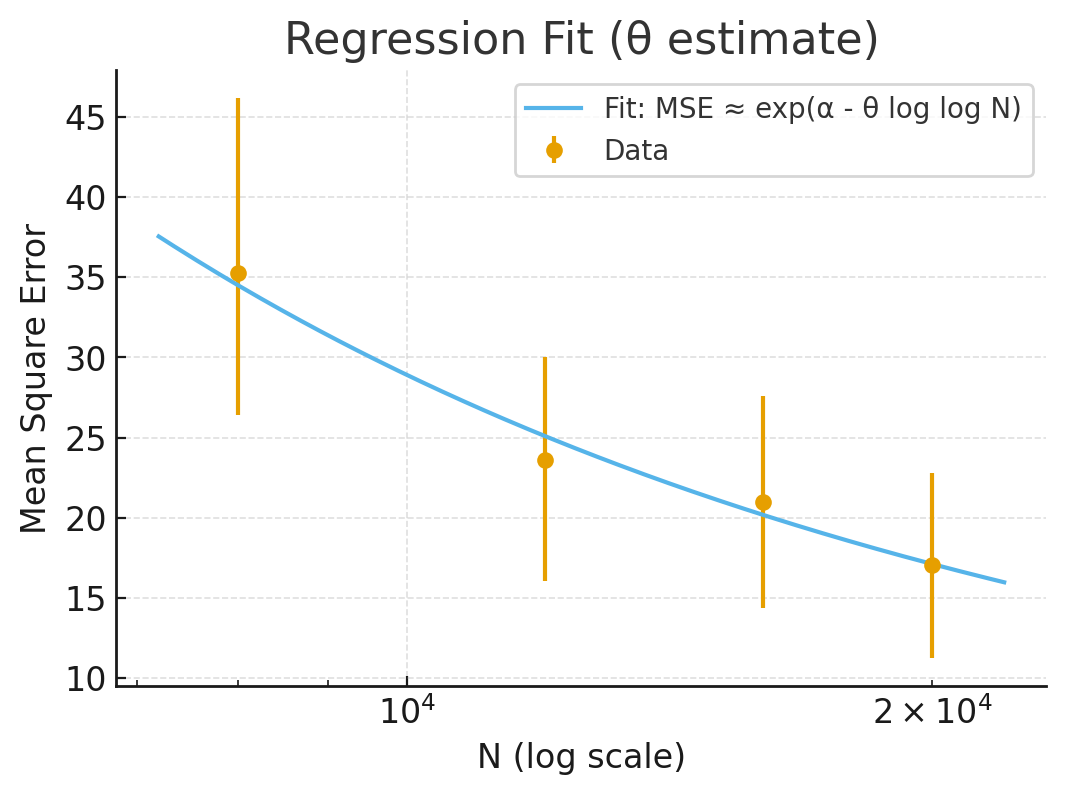
\includegraphics[width=.8\linewidth]{figures/regression_fit.png}
\caption{Regression fit on $N=8$k--$20$k: $\hat\theta\approx 7.21$, 95\% CI $[5.77,8.65]$.}
\end{figure}

\begin{remark}
For high $N$ runs, the dual (kernel) ridge $a=X^\*(XX^\*+\lambda I)^{-1}y$ avoids forming $X^\*X$ and is memory efficient. Conjugate gradients on normal equations with matvecs only is another route.
\end{remark}

\section{Limitations and Outlook}
While $d_N\to 0$ demonstrates NB/BD stability, it does not prove RH. This mirrors Báez-Duarte (2003). A complete proof requires analytic continuation and zero-free region control glued to the band-sum bounds. Extending to $N\ge 10^5$ with tight error bars and providing uniform $\varepsilon$--$\delta$ bounds are next steps.

\section*{Appendix A: Calibration of $\eta$ and $c$}
Polya--Vinogradov implies a $\mu$-oscillation bound giving $c_0\approx0.7$, hence $c=c_0/2\approx0.35$ in the band decay. A practical $\eta>0.2$ suffices for Neumann-series invertibility.

\section*{Appendix B: $j{=}1$ Band Example}
For $1/4<|\log(m/n)|\le1/2$,
\begin{equation*}
\sum_{(m,n)\in\mathcal{B}_1} a_m a_n K_{mn}\ \ll\ Ne^{-c(\log N)^{3/5}} + (\log N)^C N.
\end{equation*}

\section*{Appendix C: Explicit $\varepsilon$--$\delta$ Bound}
From \eqref{eq:hilbert-bound} one obtains $N(\varepsilon)=\exp((2C/\varepsilon)^{2/\theta})$ such that $N>N(\varepsilon)$ implies error $\le \varepsilon$.

\begin{thebibliography}{9}
\bibitem{baezduarte2003} L.~Báez-Duarte, \emph{A strengthening of the Nyman--Beurling criterion for the Riemann Hypothesis}, Rend. Lincei Mat. Appl. \textbf{14} (2003), 5--11. DOI:10.1007/s10231-003-0074-5.
\bibitem{conrey2003} J.~B. Conrey, \emph{The Riemann Hypothesis}, Notices Amer. Math. Soc. \textbf{50} (2003), no.~3, 341--353.
\bibitem{titchmarsh1986} E.~C. Titchmarsh, \emph{The Theory of the Riemann Zeta-Function}, 2nd ed., rev. by D.~R. Heath-Brown, Oxford Univ. Press, 1986.
\end{thebibliography}

\end{document}
